\documentclass[aspectratio=169]{beamer}

% Language setup
\usepackage[magyar]{babel} % Babel for Hungarian
\usepackage[T1]{fontenc} % Output character encoding
\usepackage[utf8]{inputenc} % Input character encoding
\selectlanguage{magyar}

% Beamer styling setup
\usetheme{Boadilla}
\usecolortheme{default}
%\setbeamercolor{titlelike}{parent=structure,bg=gray!15}
\setbeamertemplate{navigation symbols}{}
\setbeamertemplate{caption}[numbered]
%

% Spacing setup
\setlength{\parindent}{0pt} % No paragraph indenting
\setlength{\parskip}{5pt} % Set spacing between paragraphs
\frenchspacing
\newcommand{\mkspace}{\vspace{19pt}}
\newcommand{\rmspace}{\vspace{-19pt}}
\newcommand{\emptyline}{\vspace{\baselineskip}}
%

% Dependency setup
\usepackage{tikz}
\usetikzlibrary{decorations.markings}
\usetikzlibrary{calc}
\usepackage{caption}
\usepackage{subcaption}
%

% Style setup
\usepackage{caption}
\captionsetup{format=plain, font=scriptsize, labelformat=empty}
%

% Notation setup
\usepackage{physics} % Braket notation

% Add qi.svg logo
\usepackage{svg}
\usepackage[absolute,overlay]{textpos}

% Newline in cell
\usepackage{makecell}

\author[Nemkin Viktória, dr. Friedl Katalin]{Nemkin Viktória}
\institute[]{
\begin{small}Témavezető: dr. Friedl Katalin\end{small}
}
\title{Kvantumalgoritmusok bioinformatikai alkalmazása}
\subtitle{Protein folding \& Molecular docking}
\date{}

\begin{document}

\begin{frame}
\titlepage

\begin{textblock*}{150pt}(280pt,192pt) % {block width} (coords)
\includesvg[inkscape=overwrite,width=150pt]{./figures/qi.svg}
\end{textblock*}

\begin{textblock*}{180pt}(15pt,170pt) % {block width} (coords)
\begin{figure}[H]

\includegraphics[width=140pt]{./figures/bme_logo.pdf}
\caption{Számítástudományi és Információelméleti Tanszék}
\end{figure}

\end{textblock*}

\end{frame}

\begin{frame}{Miért foglalkozzunk bioinformatikával?}
\begin{itemize}
    \item Területek: egészségügy, gyógyszergyártás, környezetvédelem, agráripar.
    \begin{itemize}
        \item Küzdelem betegségek, globális felmelegedés, éhínség ellen.
    \end{itemize}
    \item Sok problémára nincs hatékony, egzakt algoritmus.
    \item Kvantuminformatika: új számítási modell = kvantum Turing-gép.
\end{itemize}
    
\end{frame}

\begin{frame}{Gyógyszergyártás = A rossz lyukak betömése.}


\begin{figure}[H]
  \centering
  \begin{subfigure}{.4\linewidth}
    \centering
    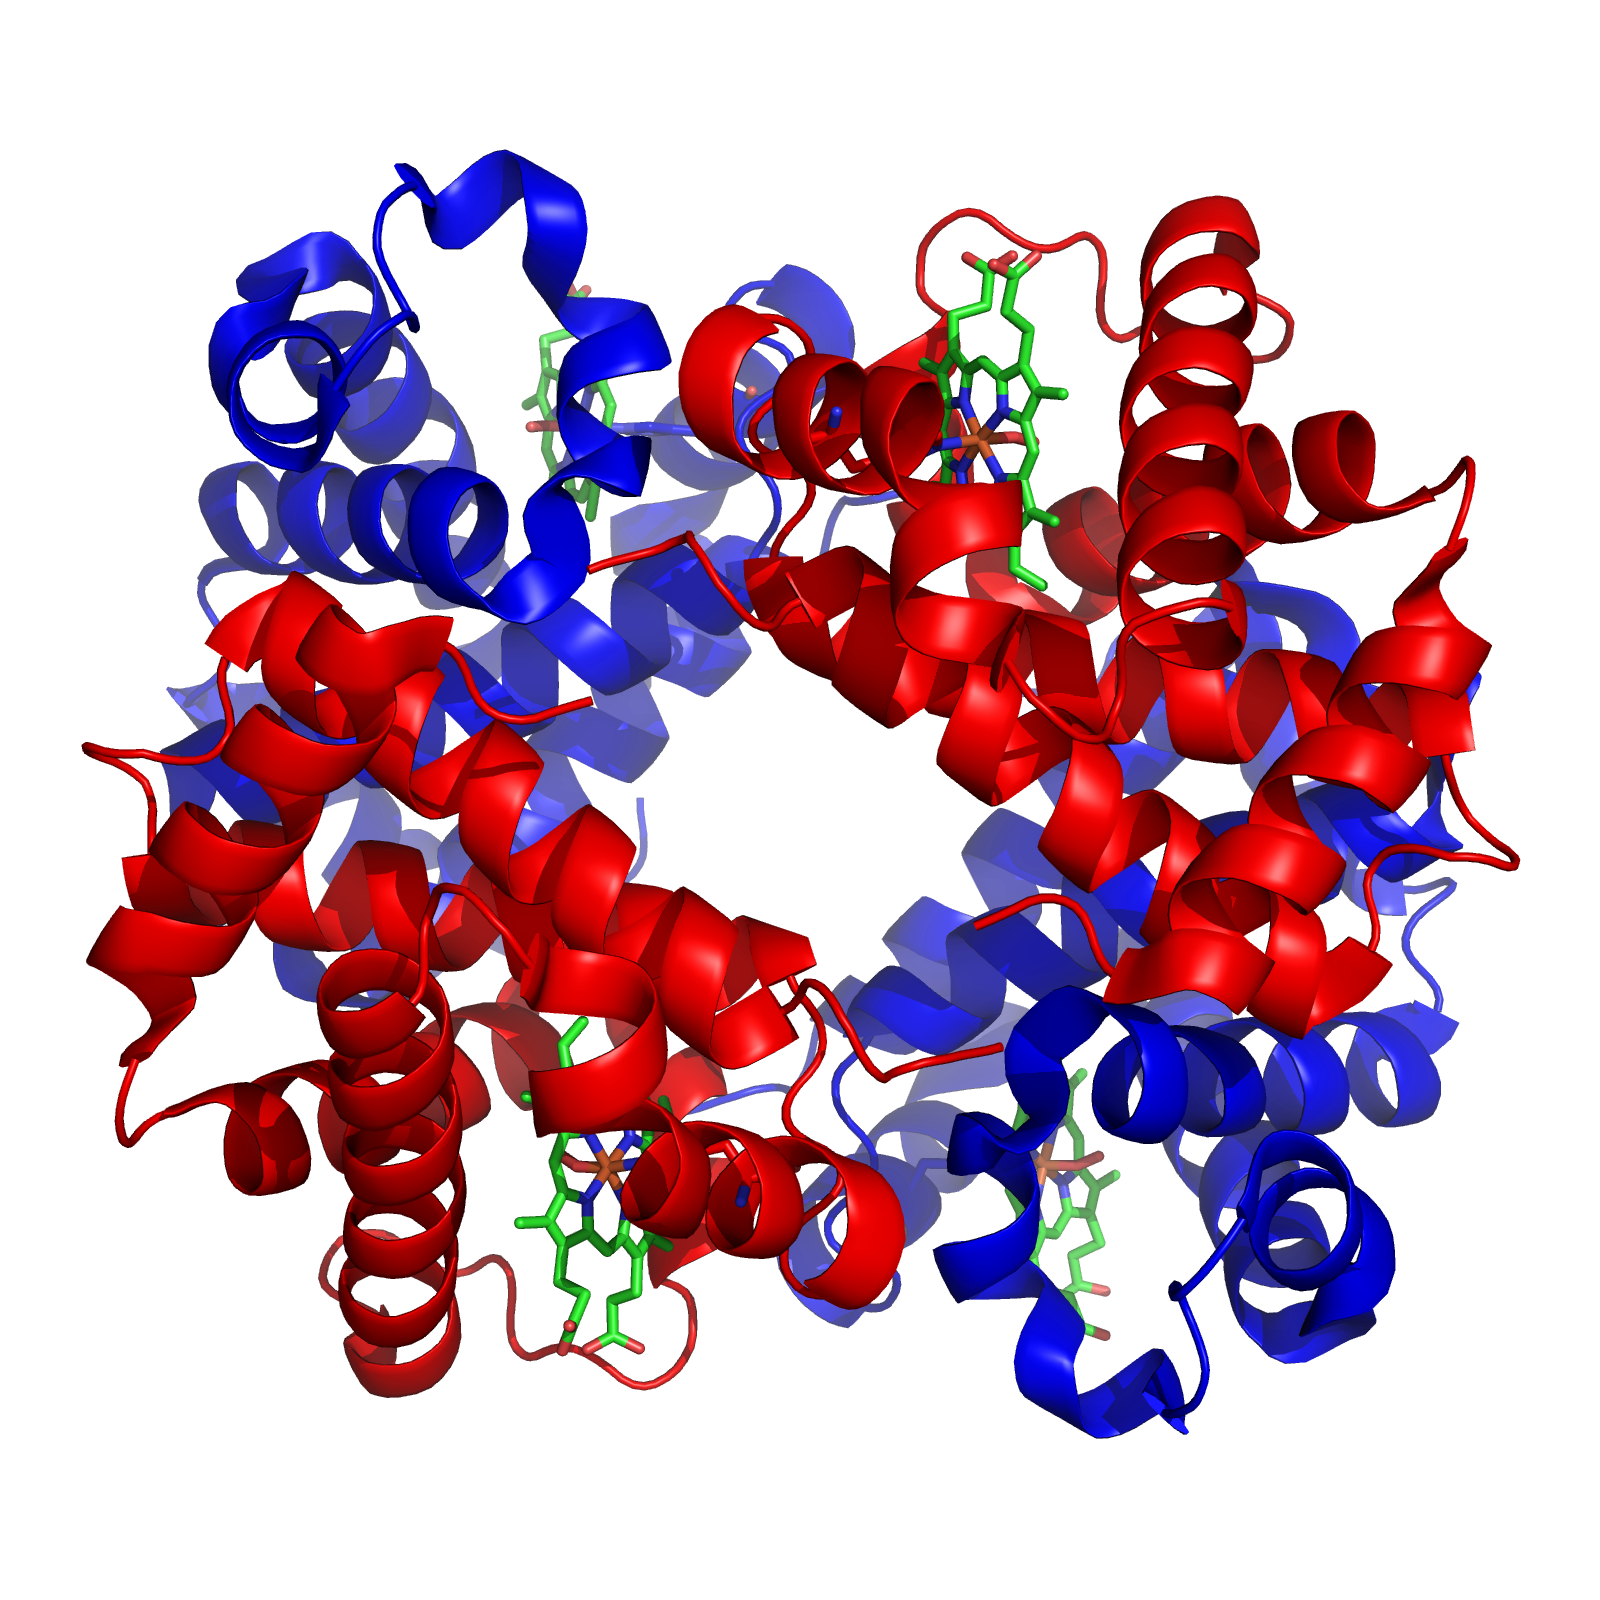
\includegraphics[width=\linewidth]{./dipterv1_figures/hemoglobin.png}
    \caption{Protein folding (Hemoglobin)}
  \end{subfigure}
  \begin{subfigure}{.48\linewidth}
    \centering
    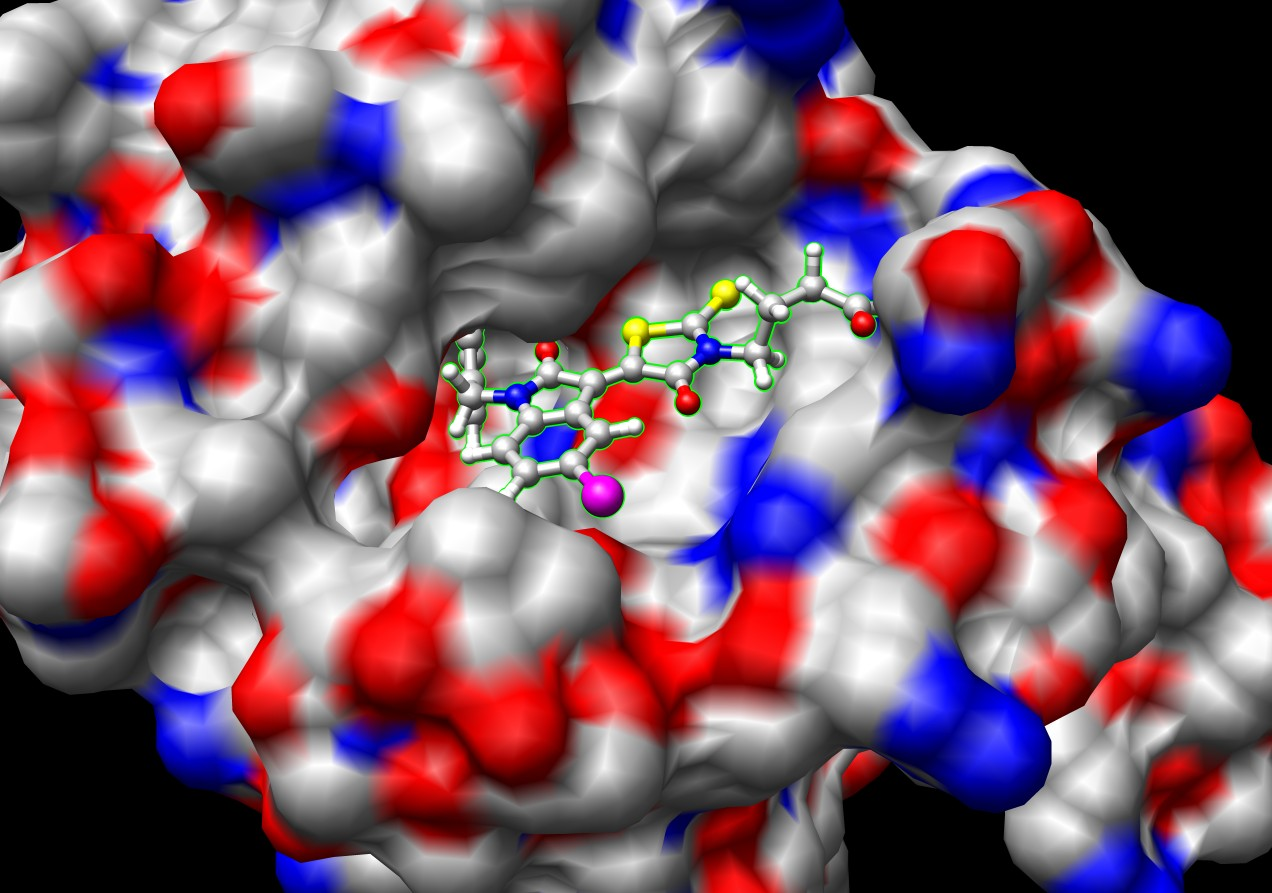
\includegraphics[width=\linewidth]{./dipterv1_figures/molecular_docking.jpg}
    \caption{Molecular docking}
  \end{subfigure}
\end{figure}

\end{frame}


\begin{frame}{Protein folding}
\begin{itemize}
    \item Proteinek = Emberi szervezet építőkövei.
    \item Feladataik: jelzés (inzulin), szállítás (hemoglobin), metabolizmus (enzimek), stb.
    \item Felépítésük: 20 lehetséges aminosavból, hosszú lánc (elsődleges struktúra).
\end{itemize}
\begin{center}
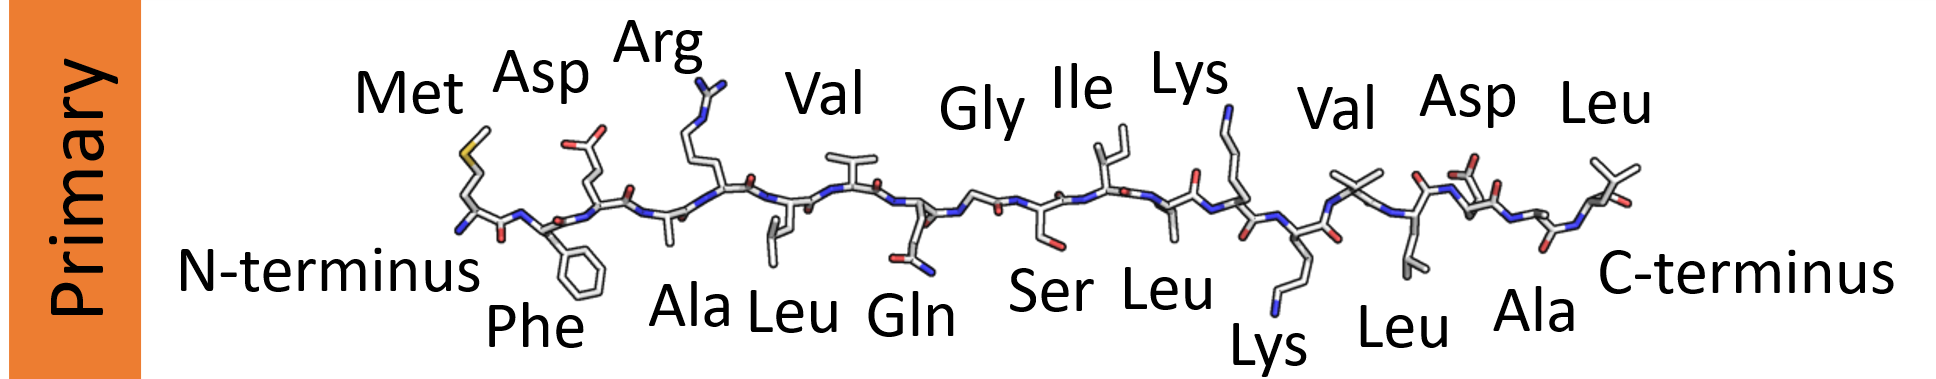
\includegraphics[width=0.8\textwidth]{dipterv1_figures/protein_structure_primary.png}
\end{center}
\end{frame}

\begin{frame}{Proteinek 4 szintű szerkezete}
\begin{center}

\includegraphics[width=0.8\textwidth]{dipterv1_figures/protein_structure_secondary.png}
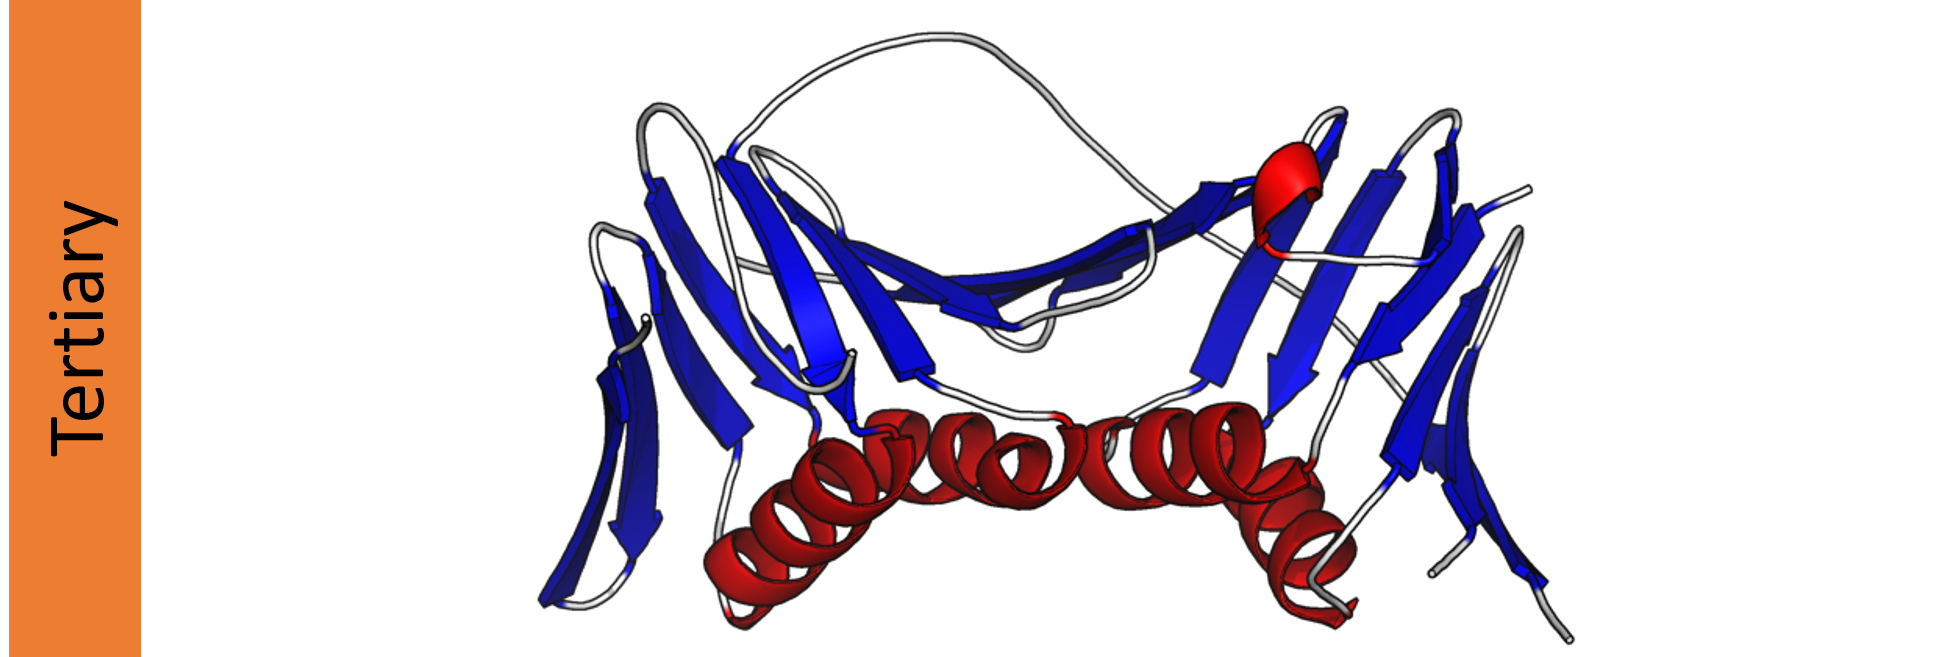
\includegraphics[width=0.8\textwidth]{dipterv1_figures/protein_structure_tertiary.png}
\end{center}
\end{frame}

\begin{frame}{Proteinek 4 szintű szerkezete}
\begin{center}
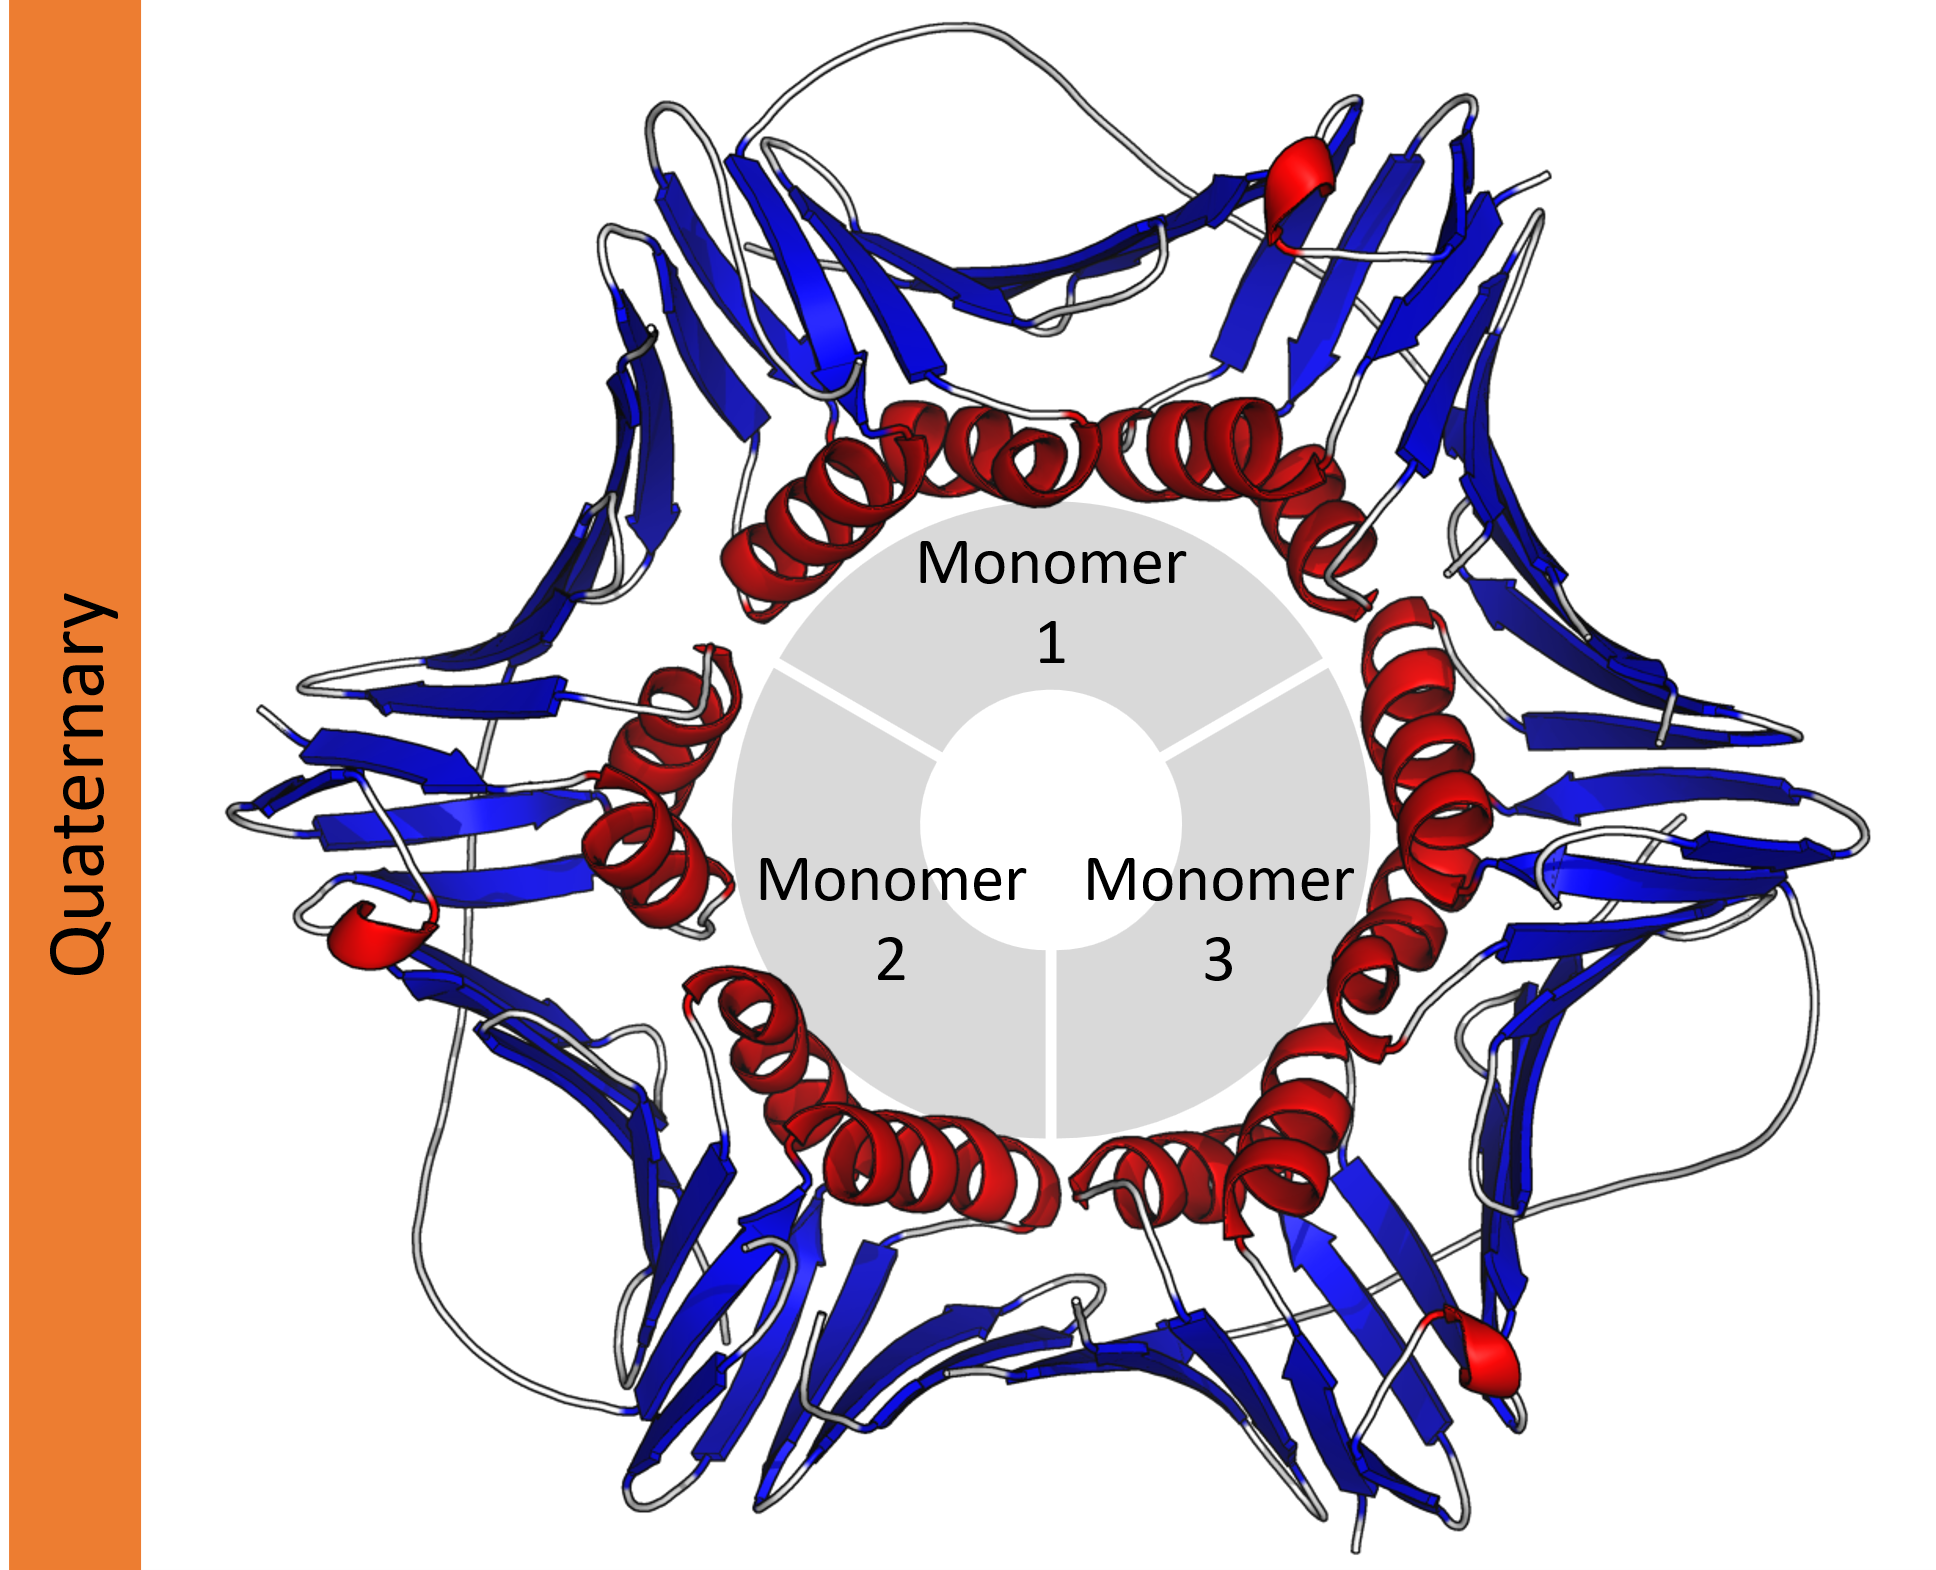
\includegraphics[width=0.6\textwidth]{dipterv1_figures/protein_structure_quaternary.png}
\end{center}
\end{frame}

\begin{frame}{Dill-féle HP modell}
\begin{itemize}
    \item Egyszerűsített modell, gyakorlatban jól használható.
    \item Aminosavak csoportosítása:
    \begin{itemize}
        \item H = Hidrofób = Apoláris = Nem szereti a vizet.
        \item P = Poláris = Hidrofil = Szereti a vizet.
        \item Sejtben víz veszi körül $\rightarrow$ kívül P, belül H.
    \end{itemize}
    \item Térbeli elhelyezkedés:
    \begin{itemize}
        \item 2D vagy 3D rács pontjaiba.
        \item Beágyazás jósága = egymás melletti H-H párok darabszáma.
    \end{itemize}
    \item Feladat: maximalizálás $\rightarrow$ bizonyítottan NP-nehéz (Hamilton-kör).
\end{itemize}
\end{frame}

\begin{frame}{HP lánc beágyazása rácsba}
\begin{figure}[H]
  \centering
  \begin{subfigure}{.4\linewidth}
    \centering
    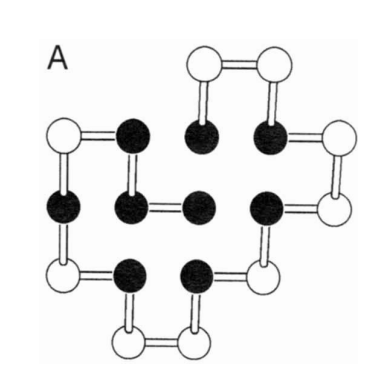
\includegraphics[width=\linewidth]{./dipterv1_figures/hp_model_2d.png}
    \caption{Beágyazás 2D rácsba}
  \end{subfigure}
  \begin{subfigure}{.55\linewidth}
    \centering
    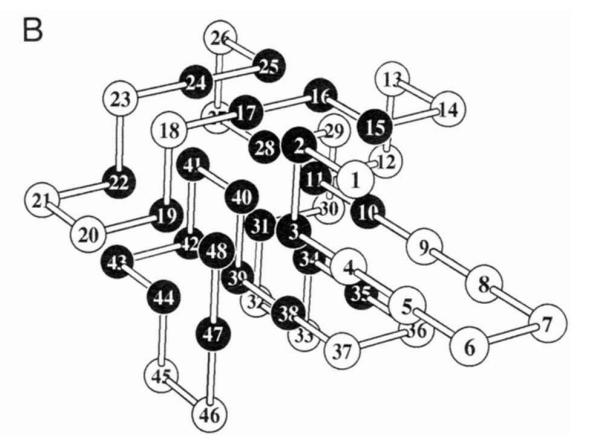
\includegraphics[width=\linewidth]{./dipterv1_figures/hp_model_3d.png}
    \caption{Beágyazás 3D rácsba}
  \end{subfigure}
  \caption{H feketével, P fehérrel jelölve}
\end{figure}
\end{frame}

\begin{frame}{Molecular docking}
\begin{itemize}
    \item Emberi test működése = kémiai reakciók $\rightarrow$ enzimek katalizátorok.
    \item Betegség = rossz kémiai reakciók $\rightarrow$ gyógyszer = enzim lyuk (kötési hely) betömése.
\end{itemize}
\begin{center}
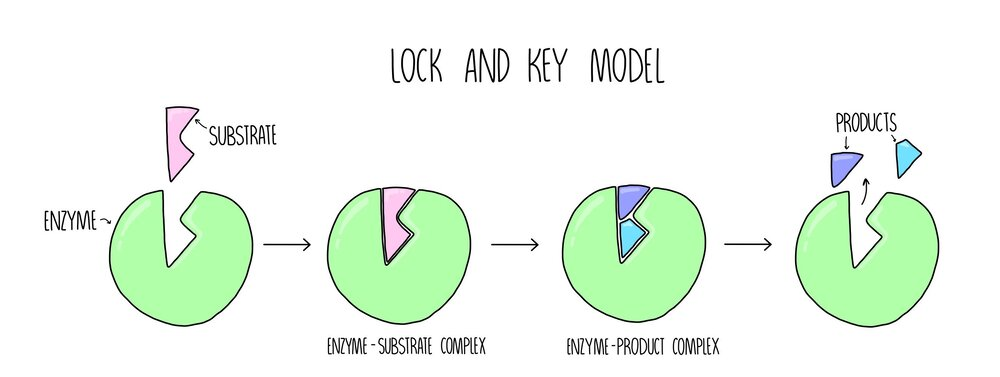
\includegraphics[width=\linewidth]{./dipterv1_figures/lock_and_key_model.jpg}
\end{center}
\end{frame}

\begin{frame}{Molecular docking}
\begin{itemize}
    \item Keressük a lyukba passzoló kulcsot.
    \item Mindkét 3D felület modellezése gráffal:
    \begin{itemize}
        \item Csúcsok = Atomok
        \item Élek = Kötések
        \item Élsúlyok = Távolságok
    \end{itemize}
    \item Feldat:
    \begin{itemize}
        \item Részgráfizomorfia $\rightarrow$ csúcsok megfeleltetése.
        \item NP-nehéz.
        \item Minimalizálandó: megfeleltetett élek súlyeltérésének szórása.
    \end{itemize}
\end{itemize}
\end{frame}

\begin{frame}{Kvantumos gyógyszergyártás}
\begin{itemize}
    \item Gyógyszergyártási feladat = \\
          Betegség $\rightarrow$ Enzim $\rightarrow$ Lyuk $\rightarrow$ Protein struktúra adatbázis $\rightarrow$ Passzoló protein
    \item Minimum / maximum keresése adatbázisban
    \item Kvantumosan:
\end{itemize}
\end{frame}

\begin{frame}{QuSZIT}
\begin{figure}
    \centering
    
\includegraphics[width=0.4\linewidth]{./dipterv1_figures/schrodingers_purple.png}
    \vspace{0.3cm}
    \caption{\huge{\href{https://cs.bme.hu/quantum/}{https://cs.bme.hu/quantum/}}}
\end{figure}
\end{frame}

\end{document}